\documentclass{article}
\usepackage{fontspec} 
\usepackage{xeCJK} 
\usepackage{ruby}
\XeTeXlinebreaklocale "zh" 
\XeTeXlinebreakskip = 0pt plus 1pt 
\renewcommand{\rubysep}{-4ex}
\pagestyle{empty}
%Select fonts
%\setmainfont[Mapping=tex-text]{Times New Roman} % rm
%\setsansfont[Mapping=tex-text]{Arial}           % sf
%\setmonofont{Courier New}                       % tt
\setCJKmainfont{DFKai-SB} %xelatex 標楷體
\setCJKmonofont{MingLiU}  %xelatex 細明體
\linespread{3}

\makeatletter
\newcommand{\rubybot}[2]{%
  \@tempdimc \f@size\p@
  \begin{tabular}[t]{@{}c@{}}
    #1\\[-3em]
    \fontsize{.8\@tempdimc}{.8\@tempdimc}\selectfont%
    \setlength{\normalbaselineskip}{0pt}#2 
  \end{tabular}%
}
\makeatother


%...
\begin{document}
中文字的測試gxiu gxiu 媠!!我
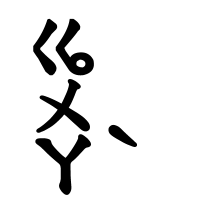
\includegraphics[height=1em]{圖/⿳⿳⿳ㆣㄨㄚˋ}
心
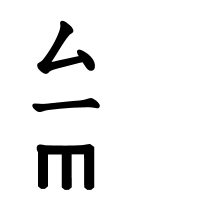
\includegraphics[height=1em]{圖/⿳⿳ㄙㄧㆬ}
\\
On this line \rubybot{aba}{がabaく}\rubybot{生}{せい}
\rubybot{我 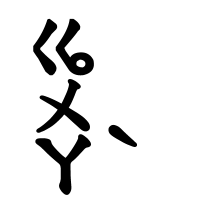
\includegraphics[height=1em]{圖/⿳⿳⿳ㆣㄨㄚˋ}}{a}
\rubybot{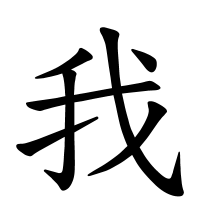
\includegraphics[height=1em]{圖/我} 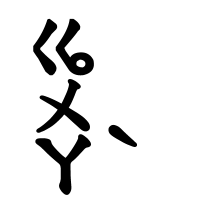
\includegraphics[height=1em]{圖/⿳⿳⿳ㆣㄨㄚˋ}}{gua2}
\rubybot{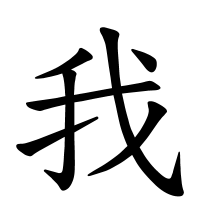
\includegraphics[height=1em]{圖/我} 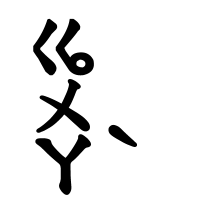
\includegraphics[height=1em]{圖/⿳⿳⿳ㆣㄨㄚˋ}}{gua2}
\rubybot{我 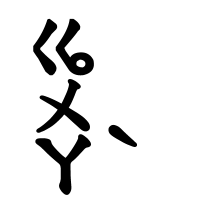
\includegraphics[height=1em]{圖/⿳⿳⿳ㆣㄨㄚˋ}}{gua2}
\rubybot{我 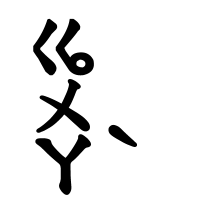
\includegraphics[height=1em]{圖/⿳⿳⿳ㆣㄨㄚˋ}}{gua2}
\rubybot{我 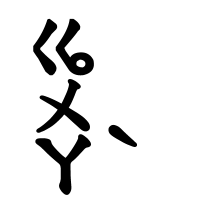
\includegraphics[height=1em]{圖/⿳⿳⿳ㆣㄨㄚˋ}}{gua2}
\rubybot{我 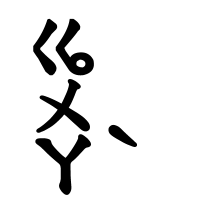
\includegraphics[height=1em]{圖/⿳⿳⿳ㆣㄨㄚˋ}}{gua2}
\rubybot{我 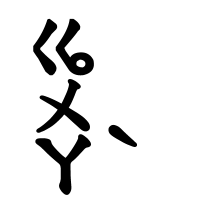
\includegraphics[height=1em]{圖/⿳⿳⿳ㆣㄨㄚˋ}}{gua2}
\rubybot{我 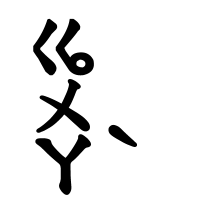
\includegraphics[height=1em]{圖/⿳⿳⿳ㆣㄨㄚˋ}}{gua2}
\rubybot{我 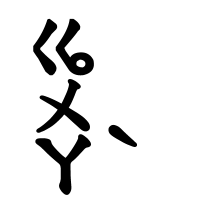
\includegraphics[height=1em]{圖/⿳⿳⿳ㆣㄨㄚˋ}}{gua2}
\rubybot{我 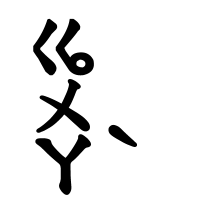
\includegraphics[height=1em]{圖/⿳⿳⿳ㆣㄨㄚˋ}}{gua2}
\rubybot{我 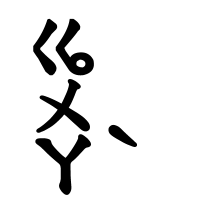
\includegraphics[height=1em]{圖/⿳⿳⿳ㆣㄨㄚˋ}}{gua2}
\rubybot{我 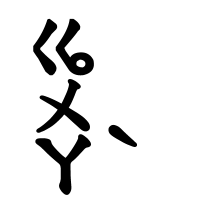
\includegraphics[height=1em]{圖/⿳⿳⿳ㆣㄨㄚˋ}}{gua2}
\rubybot{我 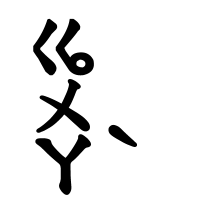
\includegraphics[height=1em]{圖/⿳⿳⿳ㆣㄨㄚˋ}}{gua2}
\rubybot{我 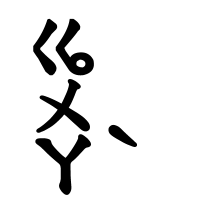
\includegraphics[height=1em]{圖/⿳⿳⿳ㆣㄨㄚˋ}}{gua2}
\rubybot{我 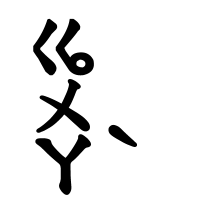
\includegraphics[height=1em]{圖/⿳⿳⿳ㆣㄨㄚˋ}}{gua2}
\rubybot{我 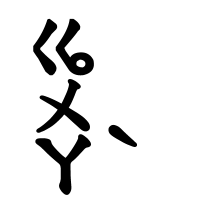
\includegraphics[height=1em]{圖/⿳⿳⿳ㆣㄨㄚˋ}}{gua2}
\rubybot{我 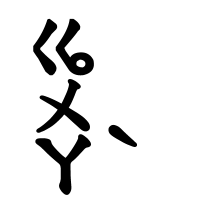
\includegraphics[height=1em]{圖/⿳⿳⿳ㆣㄨㄚˋ}}{gua2}
\rubybot{我 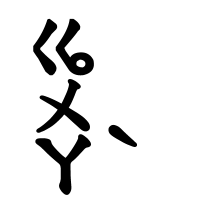
\includegraphics[height=1em]{圖/⿳⿳⿳ㆣㄨㄚˋ}}{gua2}
\rubybot{我 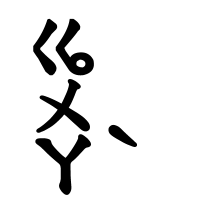
\includegraphics[height=1em]{圖/⿳⿳⿳ㆣㄨㄚˋ}}{gua2}
\rubybot{我 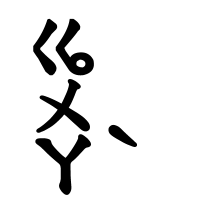
\includegraphics[height=1em]{圖/⿳⿳⿳ㆣㄨㄚˋ}}{gua2}
\rubybot{我 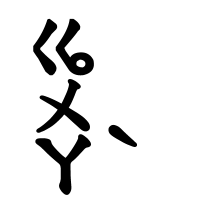
\includegraphics[height=1em]{圖/⿳⿳⿳ㆣㄨㄚˋ}}{gua2}
\rubybot{我 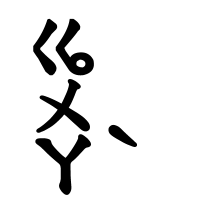
\includegraphics[height=1em]{圖/⿳⿳⿳ㆣㄨㄚˋ}}{gua2}
\rubybot{我 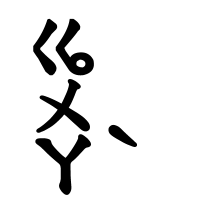
\includegraphics[height=1em]{圖/⿳⿳⿳ㆣㄨㄚˋ}}{gua2}
\rubybot{我 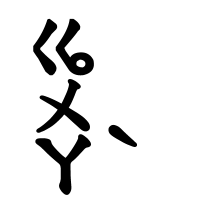
\includegraphics[height=1em]{圖/⿳⿳⿳ㆣㄨㄚˋ}}{gua2}
\rubybot{我 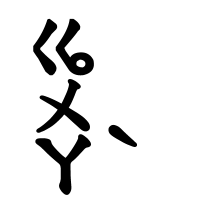
\includegraphics[height=1em]{圖/⿳⿳⿳ㆣㄨㄚˋ}}{gua2}
\\
\rubybot{我 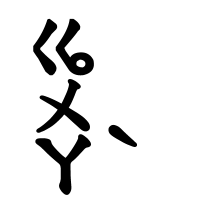
\includegraphics[height=1em]{圖/⿳⿳⿳ㆣㄨㄚˋ}}{gua2}
\rubybot{我 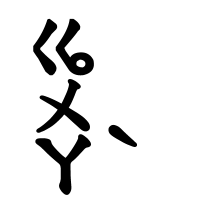
\includegraphics[height=1em]{圖/⿳⿳⿳ㆣㄨㄚˋ}}{gua2}
\rubybot{我 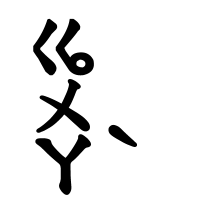
\includegraphics[height=1em]{圖/⿳⿳⿳ㆣㄨㄚˋ}}{gua2}
\rubybot{我 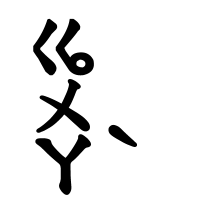
\includegraphics[height=1em]{圖/⿳⿳⿳ㆣㄨㄚˋ}}{gua2}
\rubybot{我 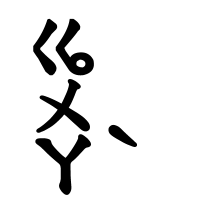
\includegraphics[height=1em]{圖/⿳⿳⿳ㆣㄨㄚˋ}}{gua2}
\rubybot{我 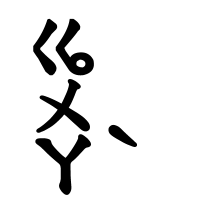
\includegraphics[height=1em]{圖/⿳⿳⿳ㆣㄨㄚˋ}}{gua2}
\rubybot{我 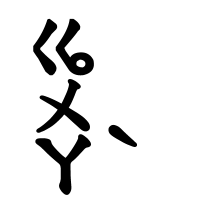
\includegraphics[height=1em]{圖/⿳⿳⿳ㆣㄨㄚˋ}}{gua2}
\rubybot{我 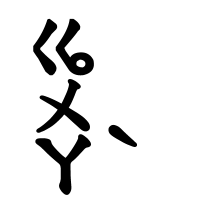
\includegraphics[height=1em]{圖/⿳⿳⿳ㆣㄨㄚˋ}}{gua2}
\rubybot{我 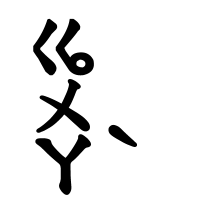
\includegraphics[height=1em]{圖/⿳⿳⿳ㆣㄨㄚˋ}}{gua2}
\rubybot{我 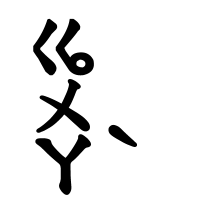
\includegraphics[height=1em]{圖/⿳⿳⿳ㆣㄨㄚˋ}}{zdom    }
\end{document}